\documentclass[10pt, dvipdfmx]{beamer}
\AtBeginDvi{\special{pdf:tounicode 90ms-RKSJ-UCS2}}
\setbeamertemplate{navigation symbols}{}
\usetheme{default}
\setbeamertemplate{footline}[frame number]
\usefonttheme{professionalfonts}
\usepackage{helvet}
\usepackage{moreverb}
\renewcommand{\familydefault}{\sfdefault}
\renewcommand{\kanjifamilydefault}{\gtdefault}
\setbeamertemplate{caption}[numbered]

\title{programming workshop}
\author{青木 聖也}
\institute[所属]{多摩美術大学情報デザイン研究室}
\date{\today}

\uselanguage{japanese}
\languagepath{japanese}

\begin{document}
    \begin{frame}[plain]
        \frametitle{}
	    \titlepage
    \end{frame}

    \begin{frame}
        \frametitle{Contents}
        \tableofcontents
    \end{frame}

%-----------------------------------------------------------
% 1日目1限:参考作品
    \section{まずはじめに}
        \begin{frame}
            \frametitle{資料について}
            今回のProgramming Workshopの資料:\\
            http://scottallen.ws/tamabi/summerworkshop2017.html\\
        \end{frame}

        \begin{frame}
            \centering{体験型の好きな作品について説明してください}
        \end{frame}

    \section{参考作品の構成要素}
        \begin{frame}
            \frametitle{単位展「りんごってこれくらい?」}
                \begin{figure}[htb]
                    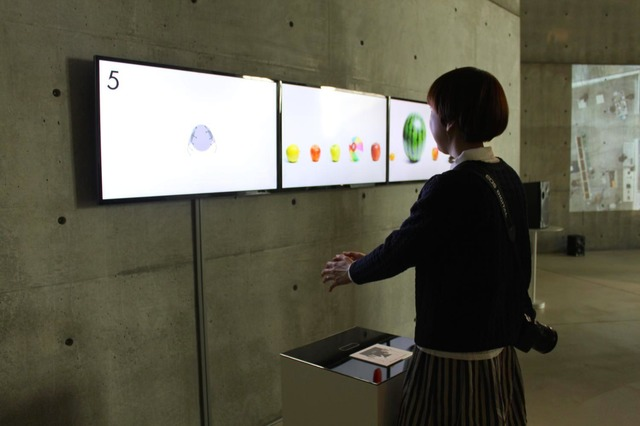
\includegraphics[width=100mm]{images/tanniten.jpg}
                    \caption{単位展「りんごってこれくらい?」体験の様子}
                    \label{fig:01}
                \end{figure}
        \end{frame}

        \begin{frame}
            \centering{実際に体験してみましょう}
        \end{frame}

        % \begin{frame}
        %     \frametitle{体験を図にすると...}
        %         \begin{figure}[htb]
        %             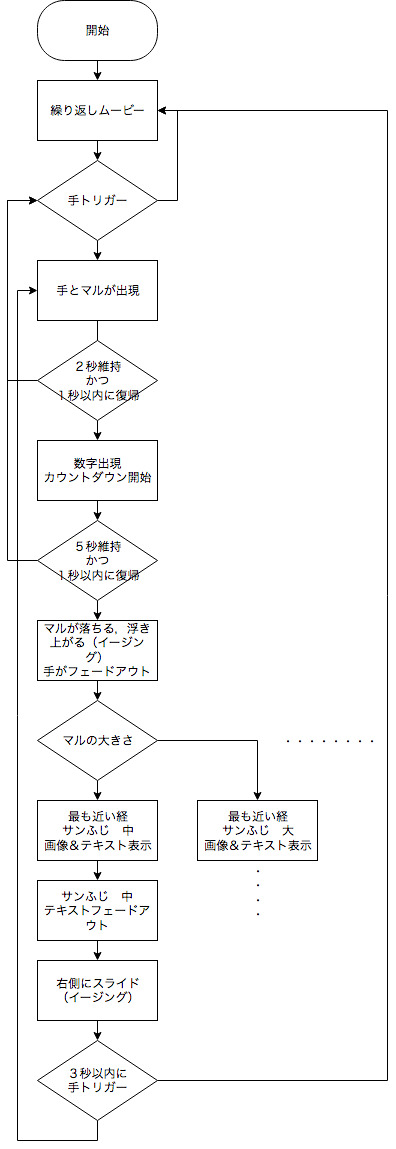
\includegraphics[height=70mm]{images/tannitenFC.jpg}
        %             \caption{体験を図にしてみた}
        %             \label{fig:02}
        %         \end{figure}
        % \end{frame}

    \section{フローチャートの書き方}
        \begin{frame}
            \frametitle{今回のサンプル}
            \begin{figure}[htb]
                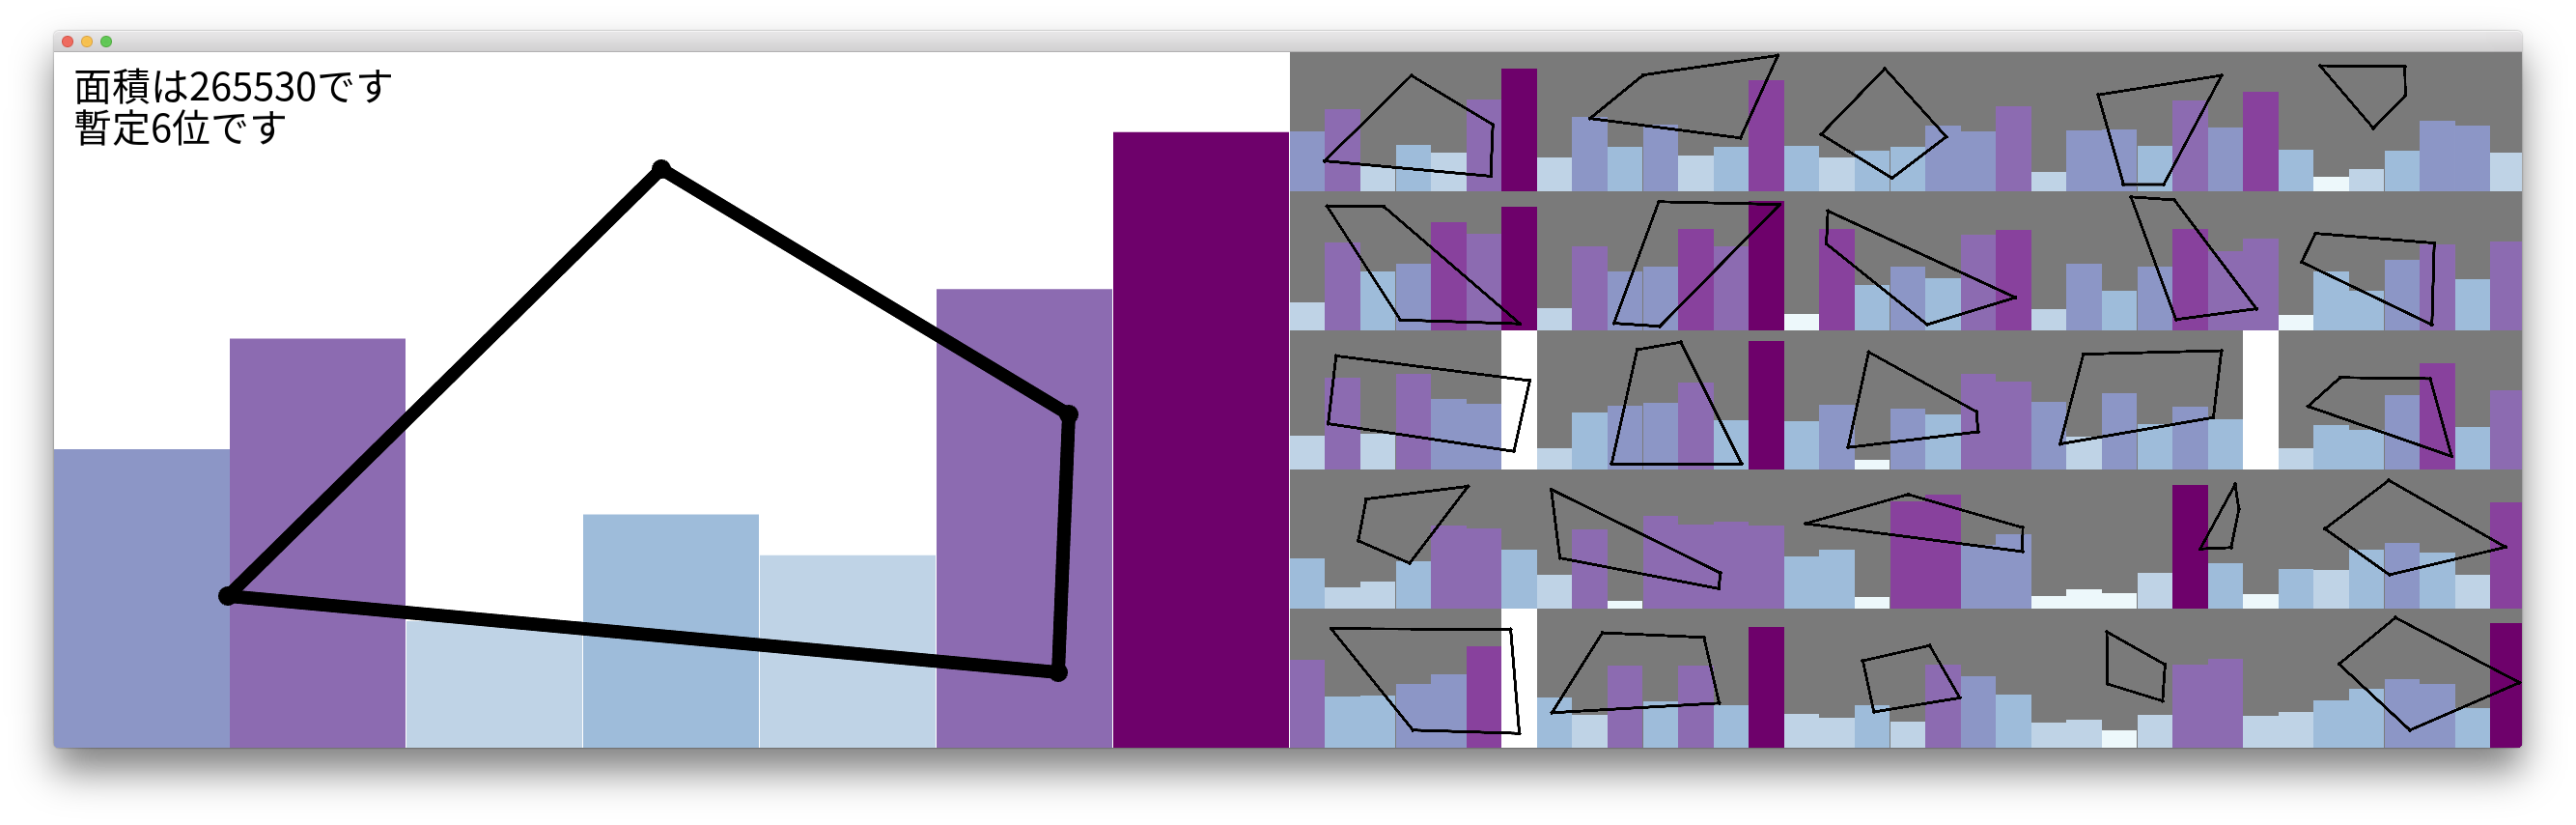
\includegraphics[width=110mm]{images/WSSample.png}
                \caption{WSSample概観}
                \label{fig:02}
            \end{figure}
        \end{frame}

    \begin{frame}
        \centering{実際に体験してみましょう}
    \end{frame}

        \begin{frame}
            \frametitle{これを図にすると}
            \begin{figure}[htb]
                 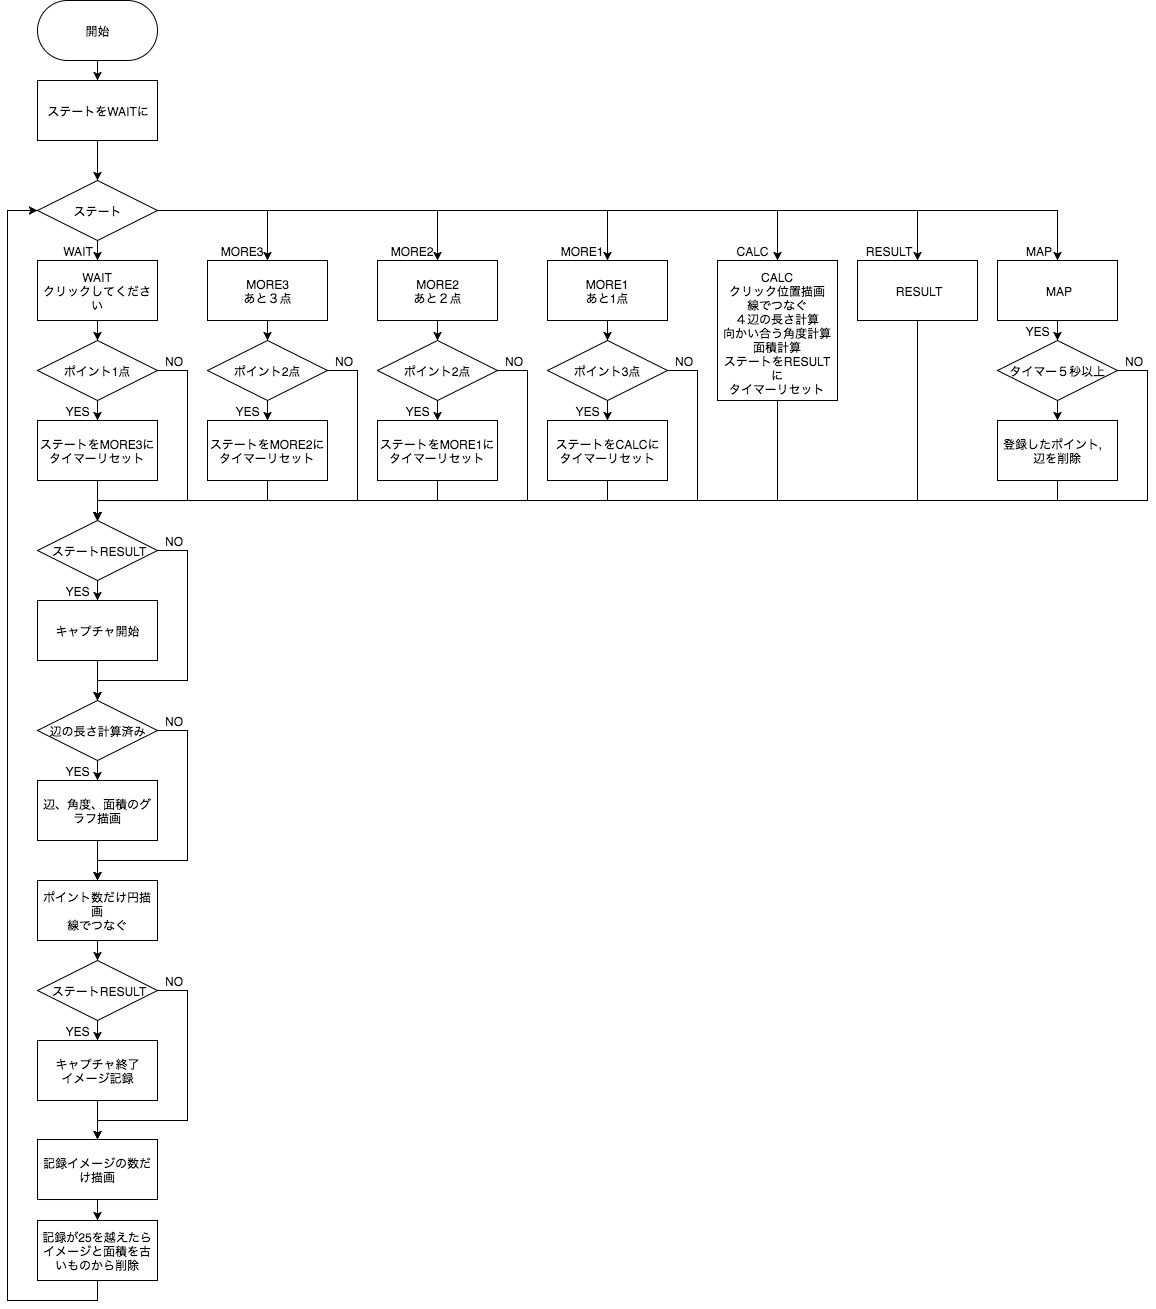
\includegraphics[height=75mm]{images/WSSampleFlowChart.jpg}
                 \caption{WSSample構造図}
                \label{fig:03}
            \end{figure}
        \end{frame}

        \begin{frame}
            \centering{この図を「フローチャート」といいます}
        \end{frame}

% 1日目2限:フローチャート
        \begin{frame}
            \frametitle{フローチャートとは}
            \begin{block}{フローチャートの特徴}
                \begin{itemize}
                    \item プロセスの各ステップを箱で表す
                    \item 流れをそれらの箱の間の矢印で表す
                    \item 様々な分野の工程の解析・設計・文書化・管理に用いられている
                \end{itemize}
            \end{block}
        \end{frame}

        \begin{frame}
            \frametitle{今回使用する環境}
            \centering{https://www.draw.io/}
            \begin{block}{draw.ioの特徴}
                \begin{itemize}
                    \item web系なのに登録など必要なし
                    \item 簡単に画像として書き出せる
                \end{itemize}
            \end{block}
        \end{frame}

        \begin{frame}
            \frametitle{draw.io}
                \begin{figure}[htb]
                    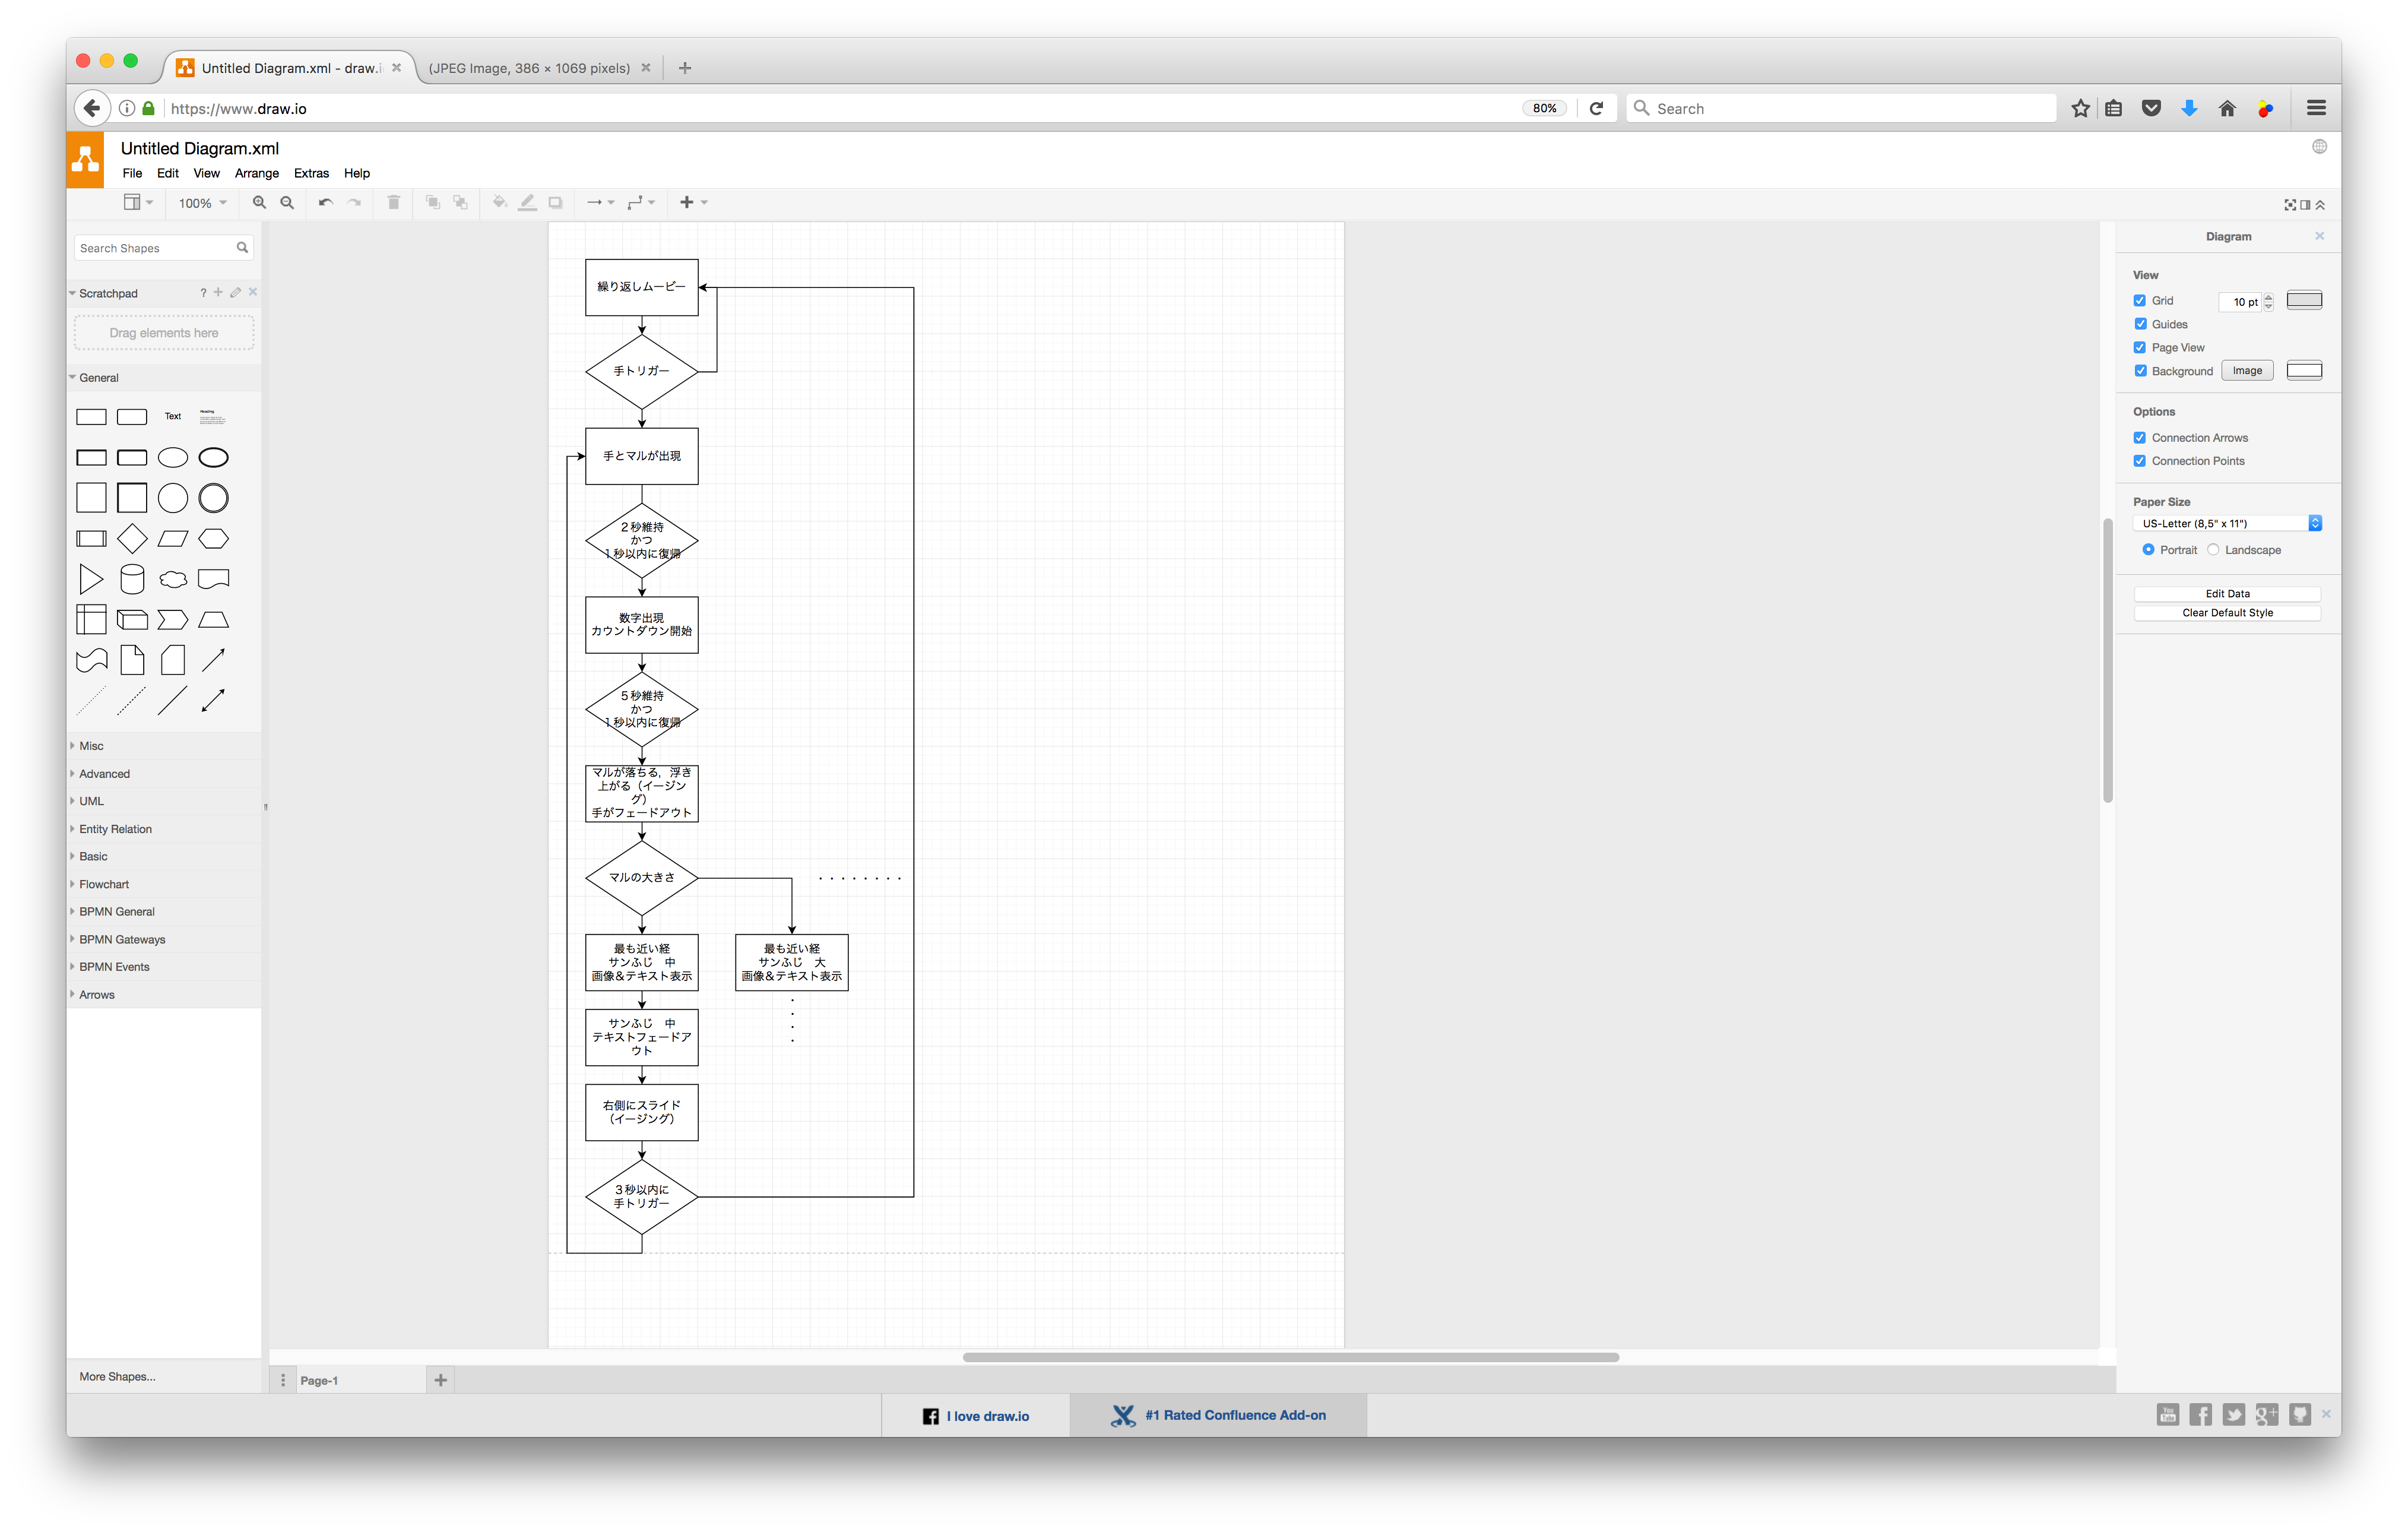
\includegraphics[width=100mm]{images/drawIO.png}
                    \caption{draw.io画面}
                    \label{fig:04}
                \end{figure}
        \end{frame}

        \begin{frame}
            \frametitle{端子}
            \begin{columns}[c]
                \begin{column}{0.50\textwidth}
                    \begin{figure}[htb]
                        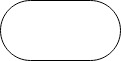
\includegraphics[height=10mm]{images/terminal.jpg}
                        \caption{端子}
                        \label{fig:05}
                    \end{figure}
                \end{column}
                \begin{column}{0.50\textwidth}
                    \begin{block}{}
                        \begin{itemize}
                            \item 開始,終了に使う
                            \item フローチャートの最初と最後に必要になる
                        \end{itemize}
                    \end{block}
                \end{column}
            \end{columns}
        \end{frame}

        \begin{frame}
            \frametitle{矢印}
            \begin{columns}[c]
                \begin{column}{0.50\textwidth}
                    \begin{figure}[htb]
                        
\includegraphics[height=10mm]{images/arrow.jpg}
                        \caption{矢印}
                        \label{fig:06}
                    \end{figure}
                \end{column}
                \begin{column}{0.50\textwidth}
                    \begin{block}{}
                        \begin{itemize}
                            \item ぷとセスとプロセスをつなぐときにつなぐ
                            \item プロセスの向きを示す
                        \end{itemize}
                    \end{block}
                \end{column}
            \end{columns}
        \end{frame}

        \begin{frame}
            \frametitle{処理}
            \begin{columns}[c]
                \begin{column}{0.50\textwidth}
                    \begin{figure}[htb]
                        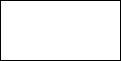
\includegraphics[height=10mm]{images/processing.jpg}
                        \caption{処理}
                        \label{fig:07}
                    \end{figure}
                \end{column}
                \begin{column}{0.50\textwidth}
                    \begin{block}{}
                        \begin{itemize}
                            \item 処理があるとき使う
                            \item 「1足す」「画像を表示する」など
                        \end{itemize}
                    \end{block}
                \end{column}
            \end{columns}
        \end{frame}

        \begin{frame}
            \frametitle{判断}
            \begin{columns}[c]
                \begin{column}{0.50\textwidth}
                    \begin{figure}[htb]
                        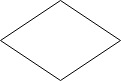
\includegraphics[height=10mm]{images/judge.jpg}
                        \caption{判断}
                        \label{fig:08}
                    \end{figure}
                \end{column}
                \begin{column}{0.50\textwidth}
                    \begin{block}{}
                        \begin{itemize}
                            \item 選択肢が2つ以上あるとき使う
                            \item 「タイプした文字」: 「'a'」「'b'」など
                        \end{itemize}
                    \end{block}
                \end{column}
            \end{columns}
        \end{frame}

        \begin{frame}
            \frametitle{ループ}
            \begin{columns}[c]
                \begin{column}{0.50\textwidth}
                    \begin{figure}[htb]
                        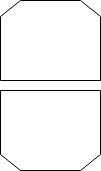
\includegraphics[height=25mm]{images/loop.jpg}
                        \caption{ループ}
                        \label{fig:09}
                    \end{figure}
                \end{column}
                \begin{column}{0.50\textwidth}
                    \begin{block}{}
                        \begin{itemize}
                            \item 繰り返し行なう処理があるとき使う
                            \item 「円が10個できたら終了」など
                        \end{itemize}
                    \end{block}
                \end{column}
            \end{columns}
        \end{frame}

        \begin{frame}
            \frametitle{もう一度フローチャートを見てみる}
            \begin{figure}[htb]
                 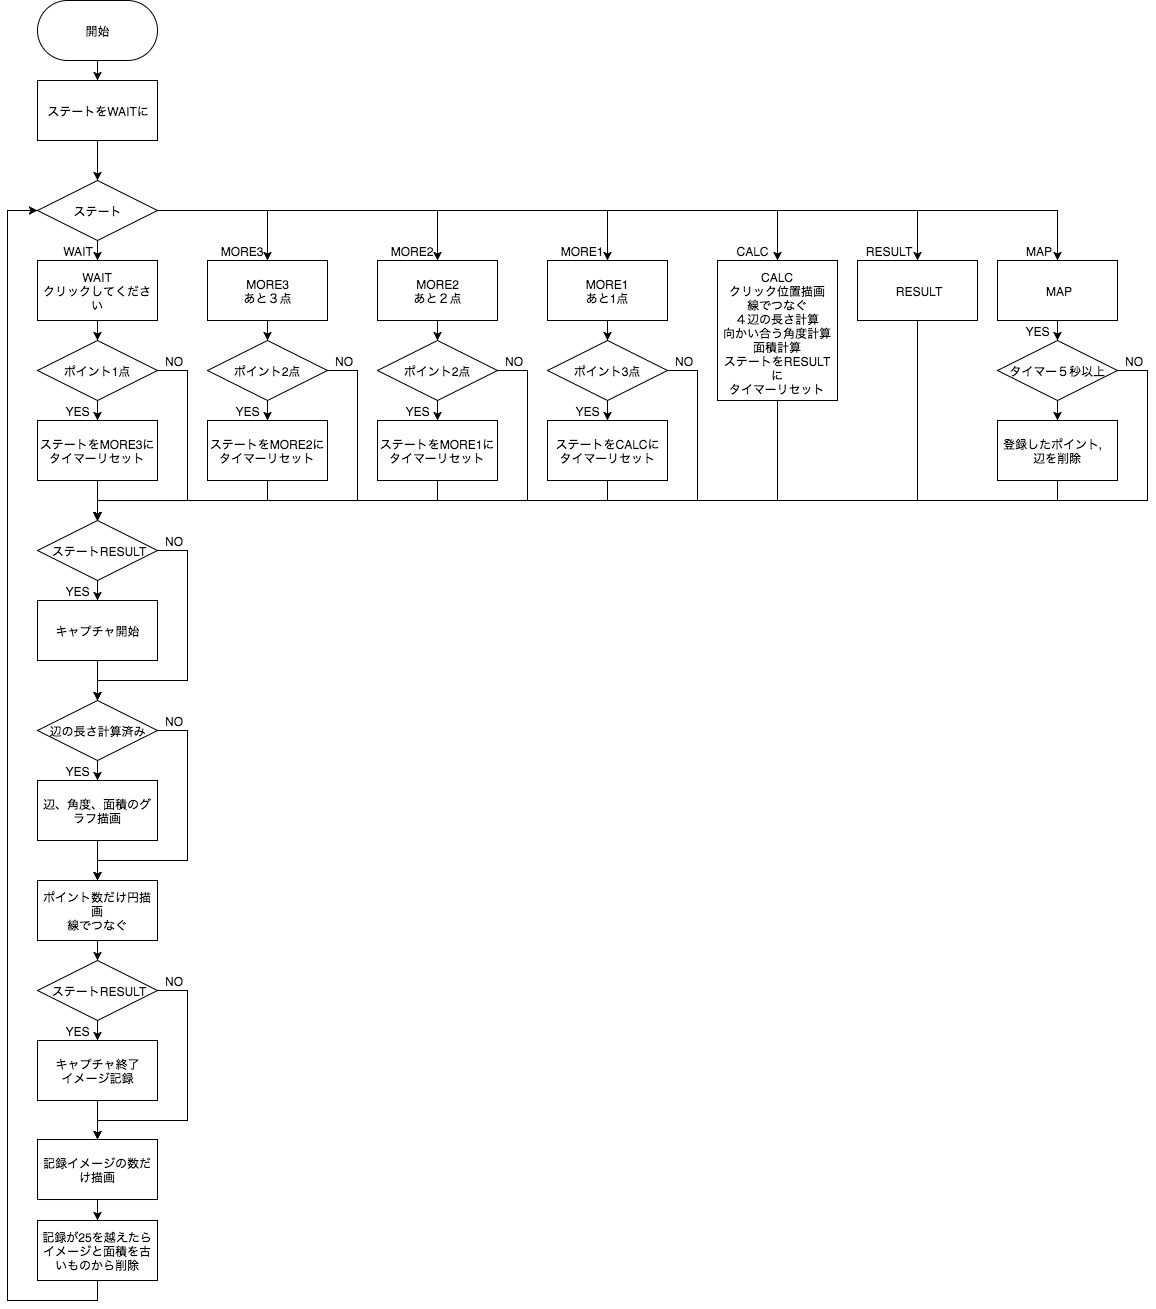
\includegraphics[height=75mm]{images/WSSampleFlowChart.jpg}
                 \caption{WSSampleフローチャート}
                \label{fig:10}
            \end{figure}
        \end{frame}

        \begin{frame}
            \centering{作りたい作品をスケッチしてみましょう}
        \end{frame}

        \begin{frame}
            \centering{共有タイム}
        \end{frame}

% 1日目3,4限:oFレクチャー
    \section{openFrameworksを用いた体験型アプリの書き方}
        \begin{frame}
            \frametitle{ステートを切り替える WS01enum/}
            \begin{figure}[htb]
                 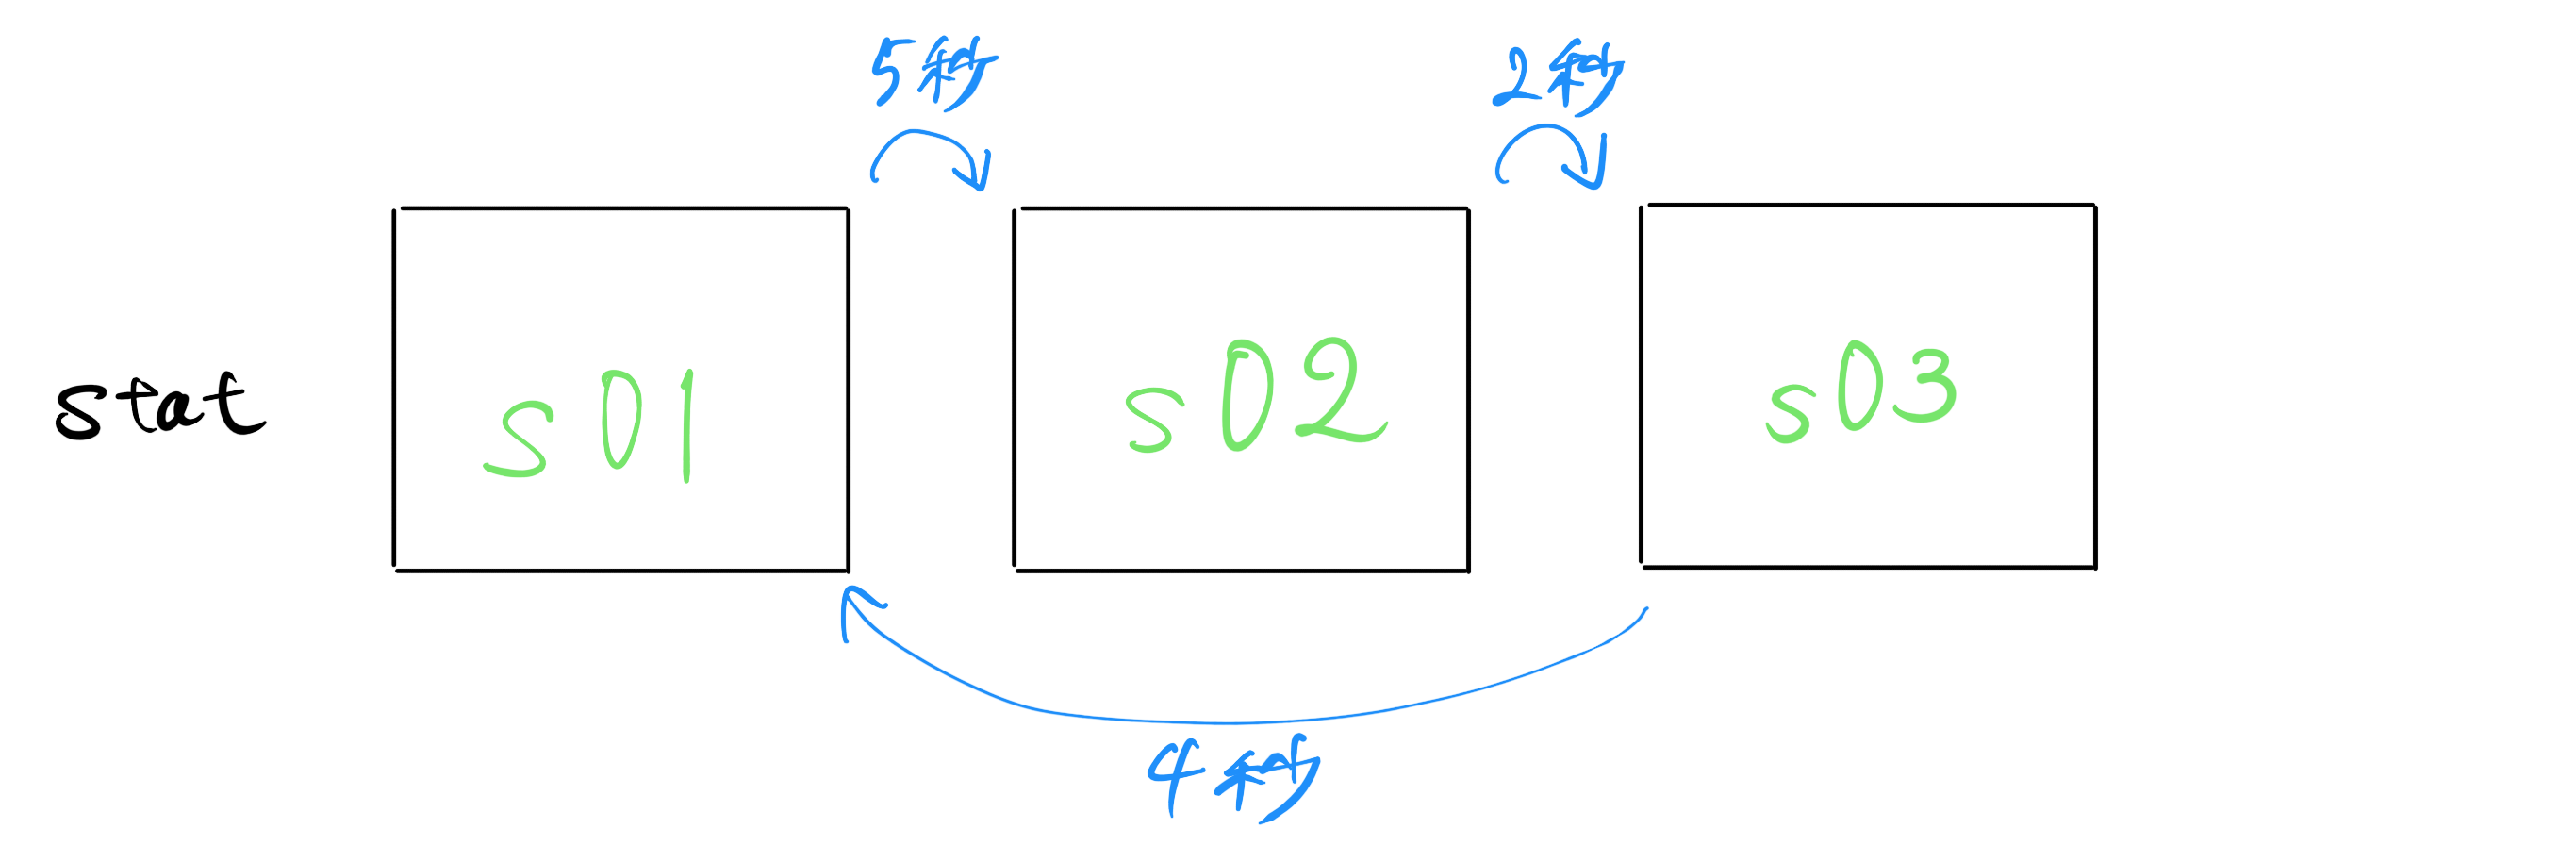
\includegraphics[width=110mm]{images/ws01-1.png}
                 \caption{WS01ステータス移行図解}
                \label{fig:11}
            \end{figure}
        \end{frame}

        \begin{frame}
            \frametitle{ステートを切り替える WS01enum/}
            \begin{figure}[htb]
                 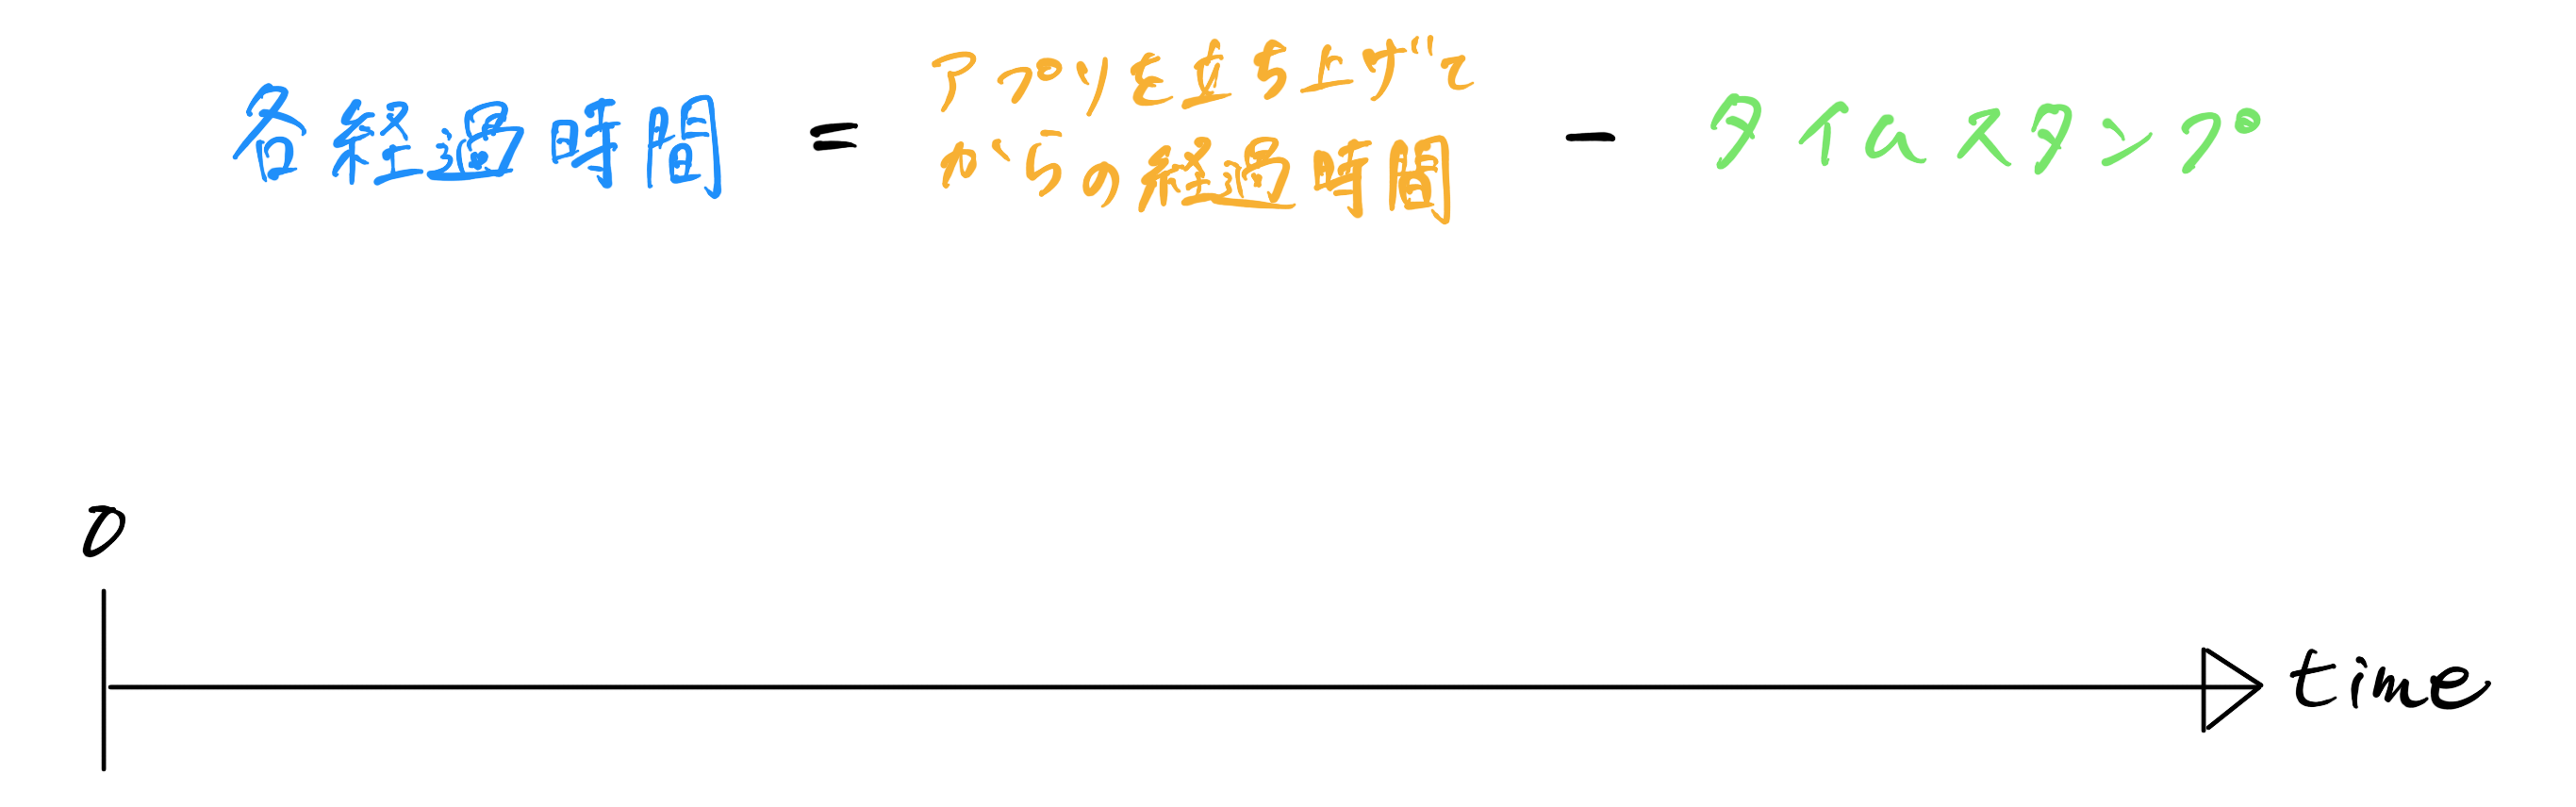
\includegraphics[width=110mm]{images/ws01-2.png}
                 \caption{WS01時間軸図解}
                \label{fig:12}
            \end{figure}
        \end{frame}

        % \begin{frame}
        %     \frametitle{ステートを切り替える WS01enum/}
        %     \begin{columns}[c]
        %         \begin{column}{0.60\textwidth}
        %             \tiny
        %             WS01enum/src/ofApp.cpp
        %             % \scriptsize
        %             % \tiny
        %             \fontsize{3.5pt}{0pt}\selectfont
        %             \verbatimtabinput{../WS01enum/src/ofApp.cpp}
        %         \end{column}
        %         \begin{column}{0.40\textwidth}
        %             \tiny
        %             WS01enum/src/ofApp.h
        %             % \scriptsize
        %             \fontsize{3.5pt}{0pt}\selectfont
        %             \verbatimtabinput{../WS01enum/src/ofApp.h}
        %         \end{column}
        %     \end{columns}
        % \end{frame}

        \begin{frame}
            \frametitle{サウンド、ビデオを扱う WS02SoundVideo/}
            \begin{figure}[htb]
                 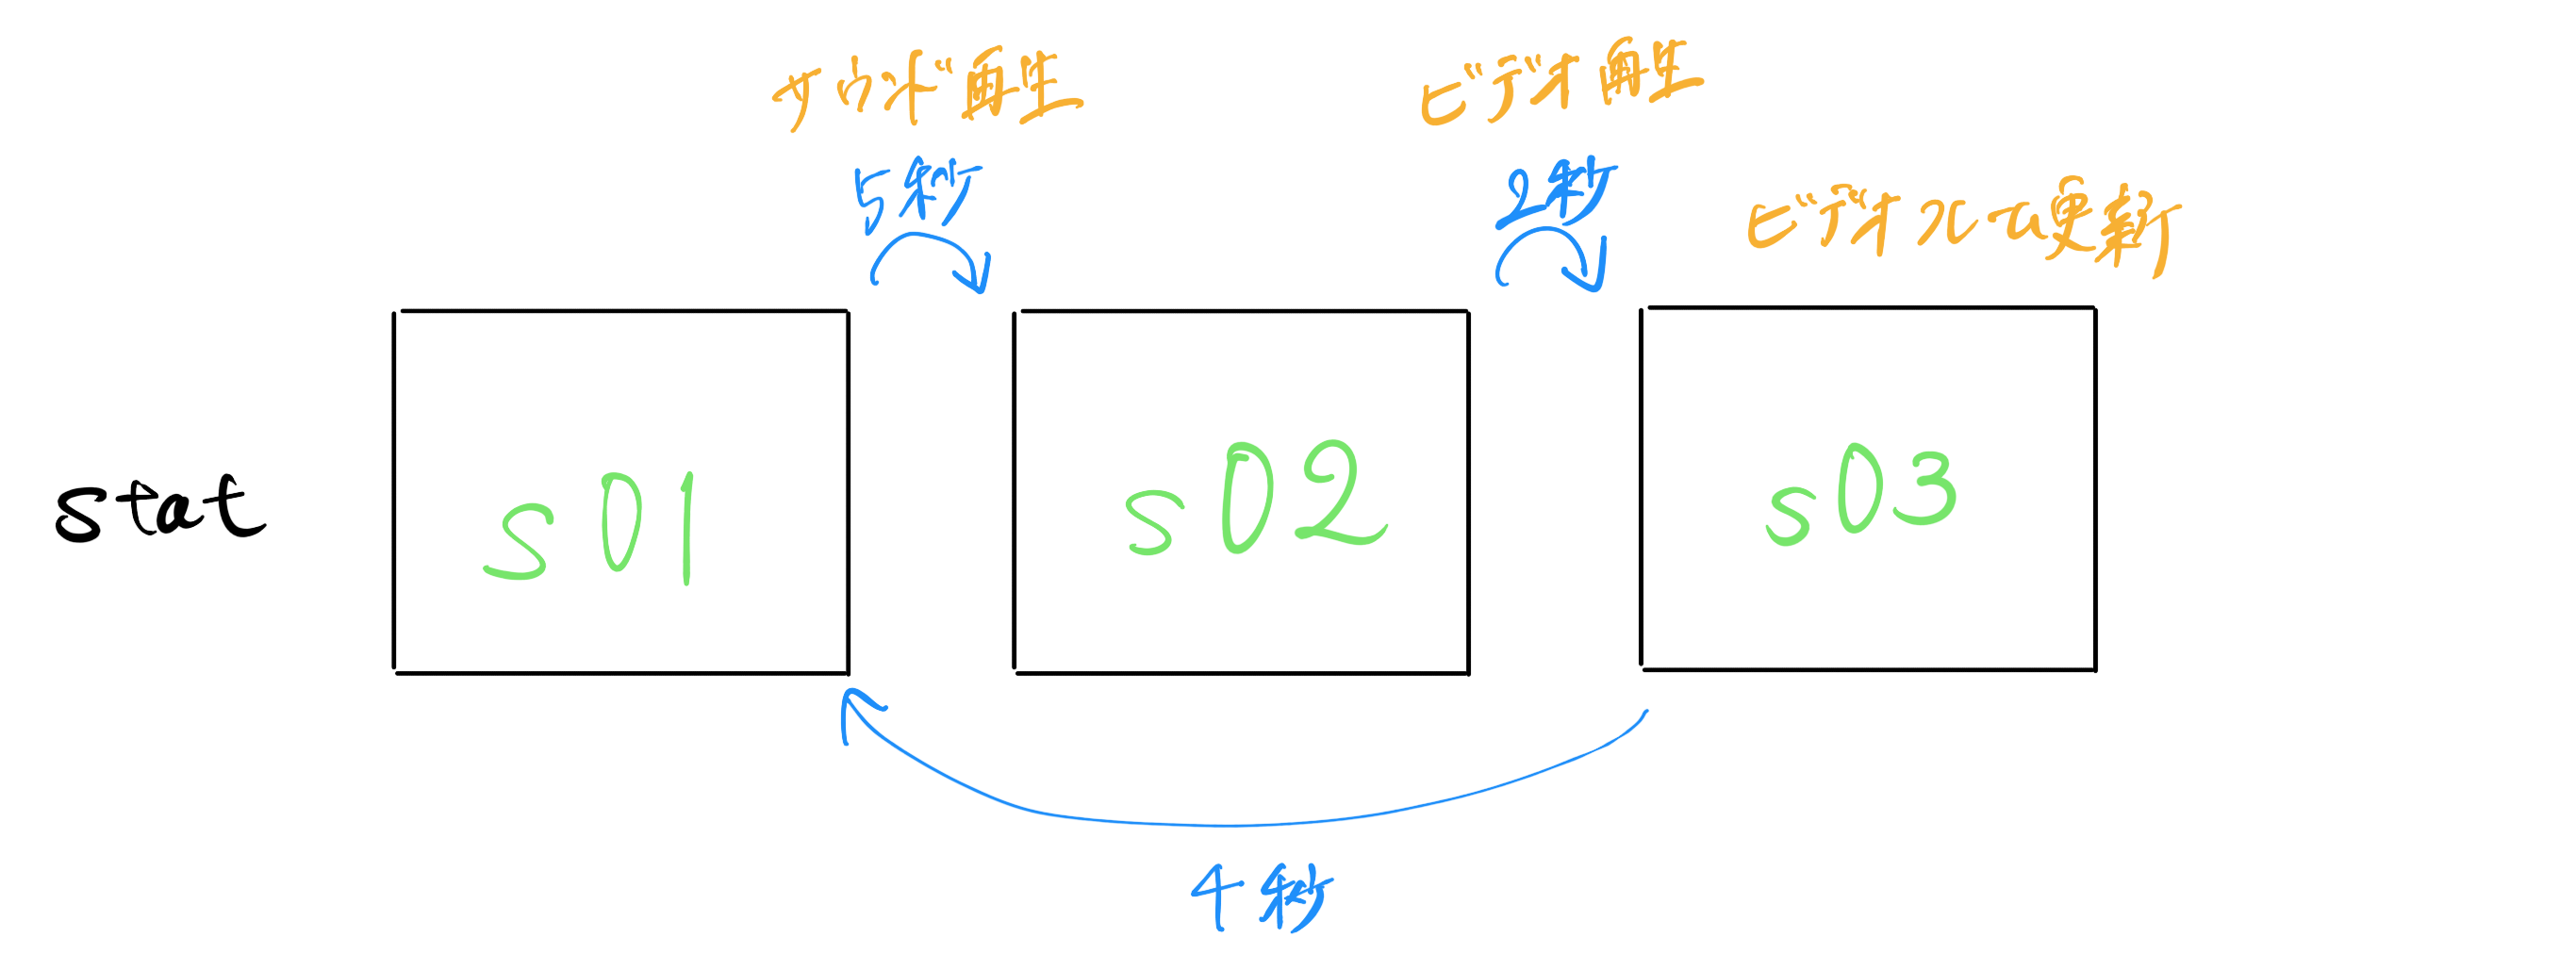
\includegraphics[width=110mm]{images/ws02-1.png}
                 \caption{WS02ステータス移行図解}
                \label{fig:13}
            \end{figure}
        \end{frame}

        \begin{frame}
            \frametitle{トリガーする,ロスト時に消去 WS03TriggerLost/}
            \begin{figure}[htb]
                 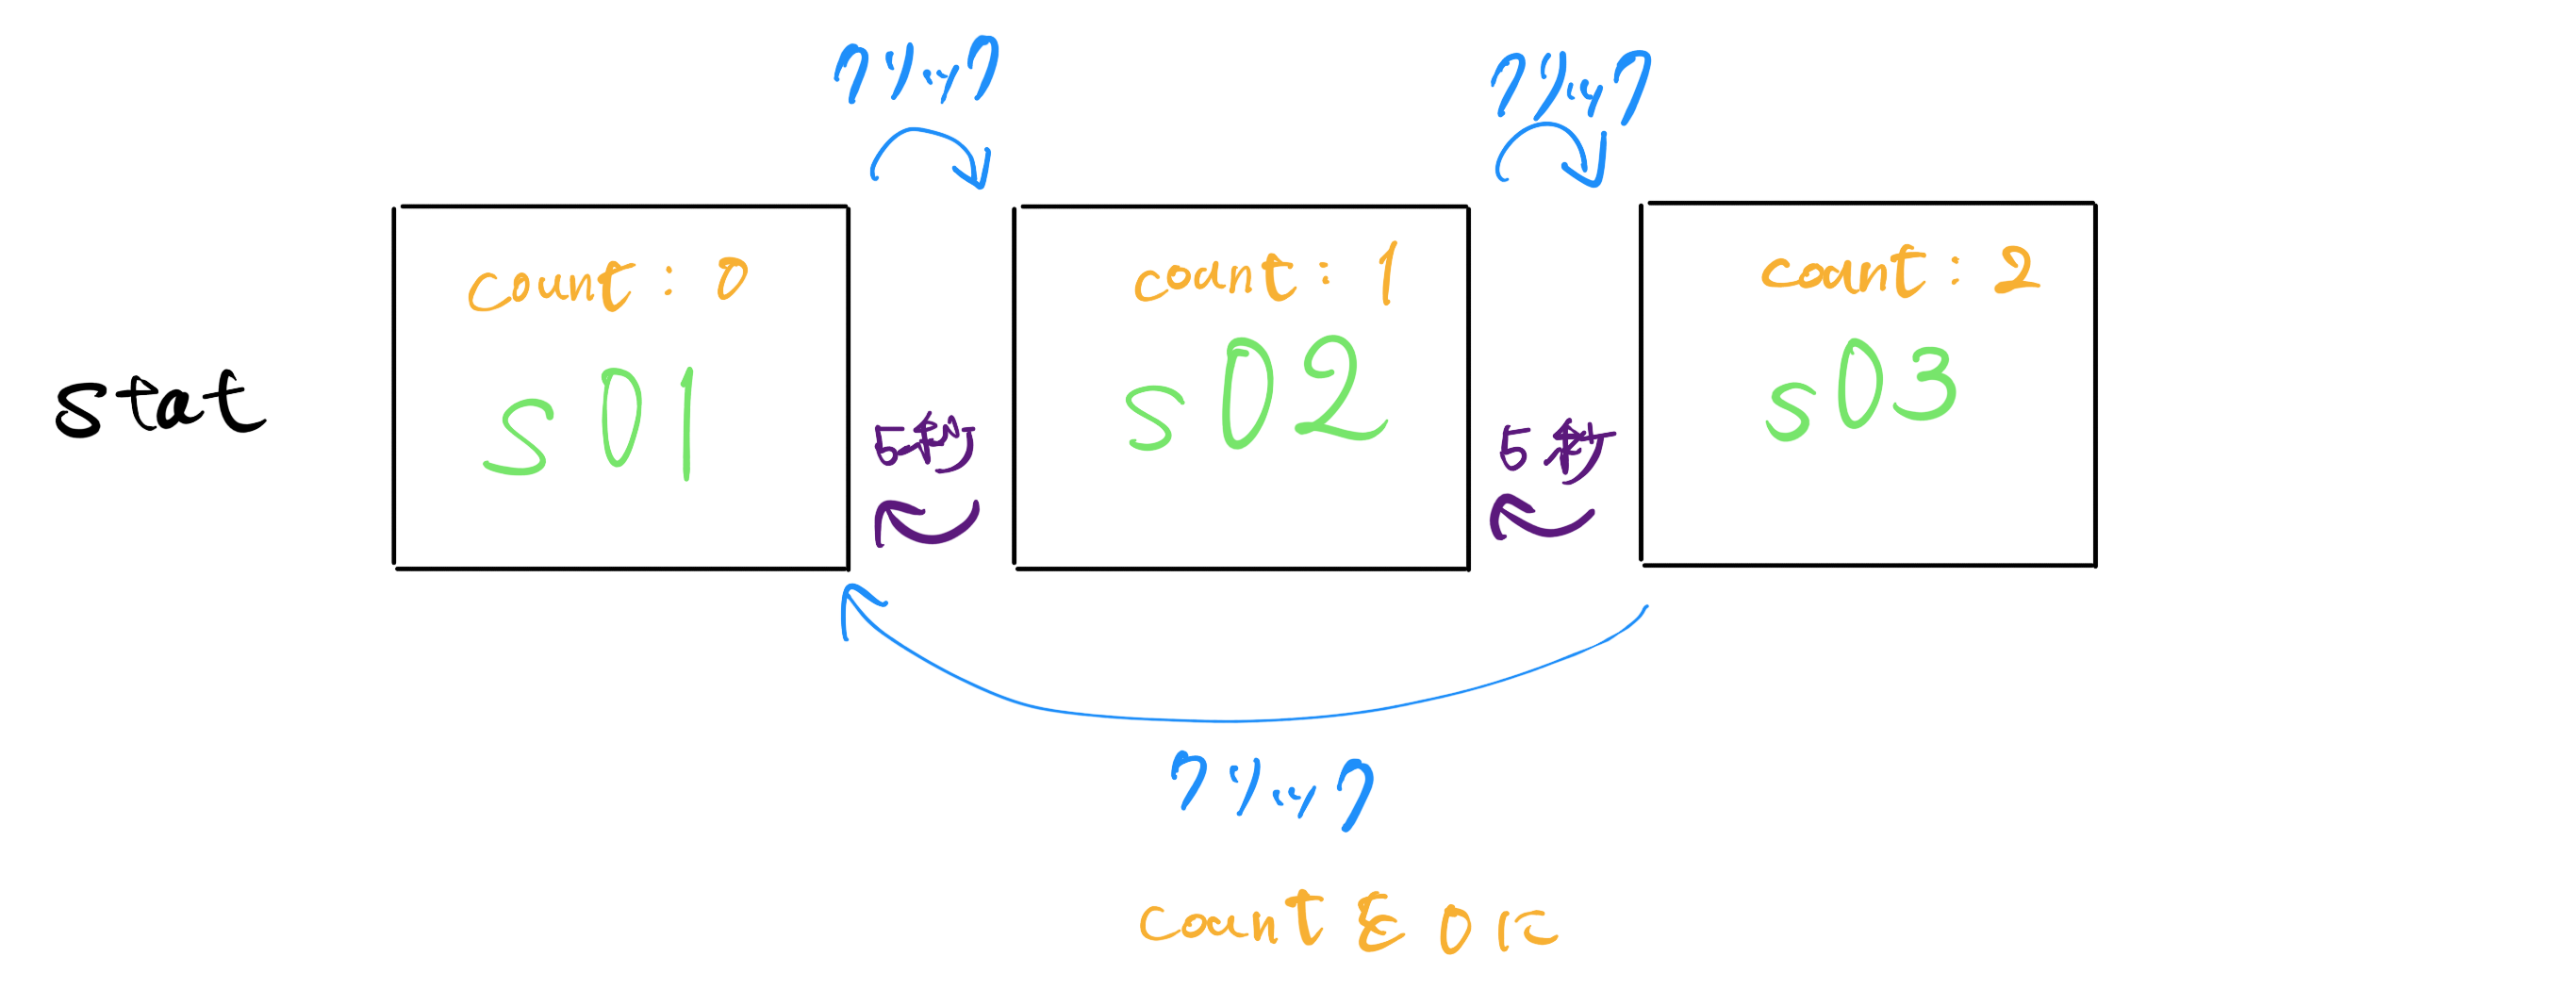
\includegraphics[width=110mm]{images/ws03-1.png}
                 \caption{WS03ステータス移行図解}
                \label{fig:14}
            \end{figure}
        \end{frame}

        \begin{frame}
            \frametitle{記録する,比べる WS04RecordCompare/}
            \begin{figure}[htb]
                 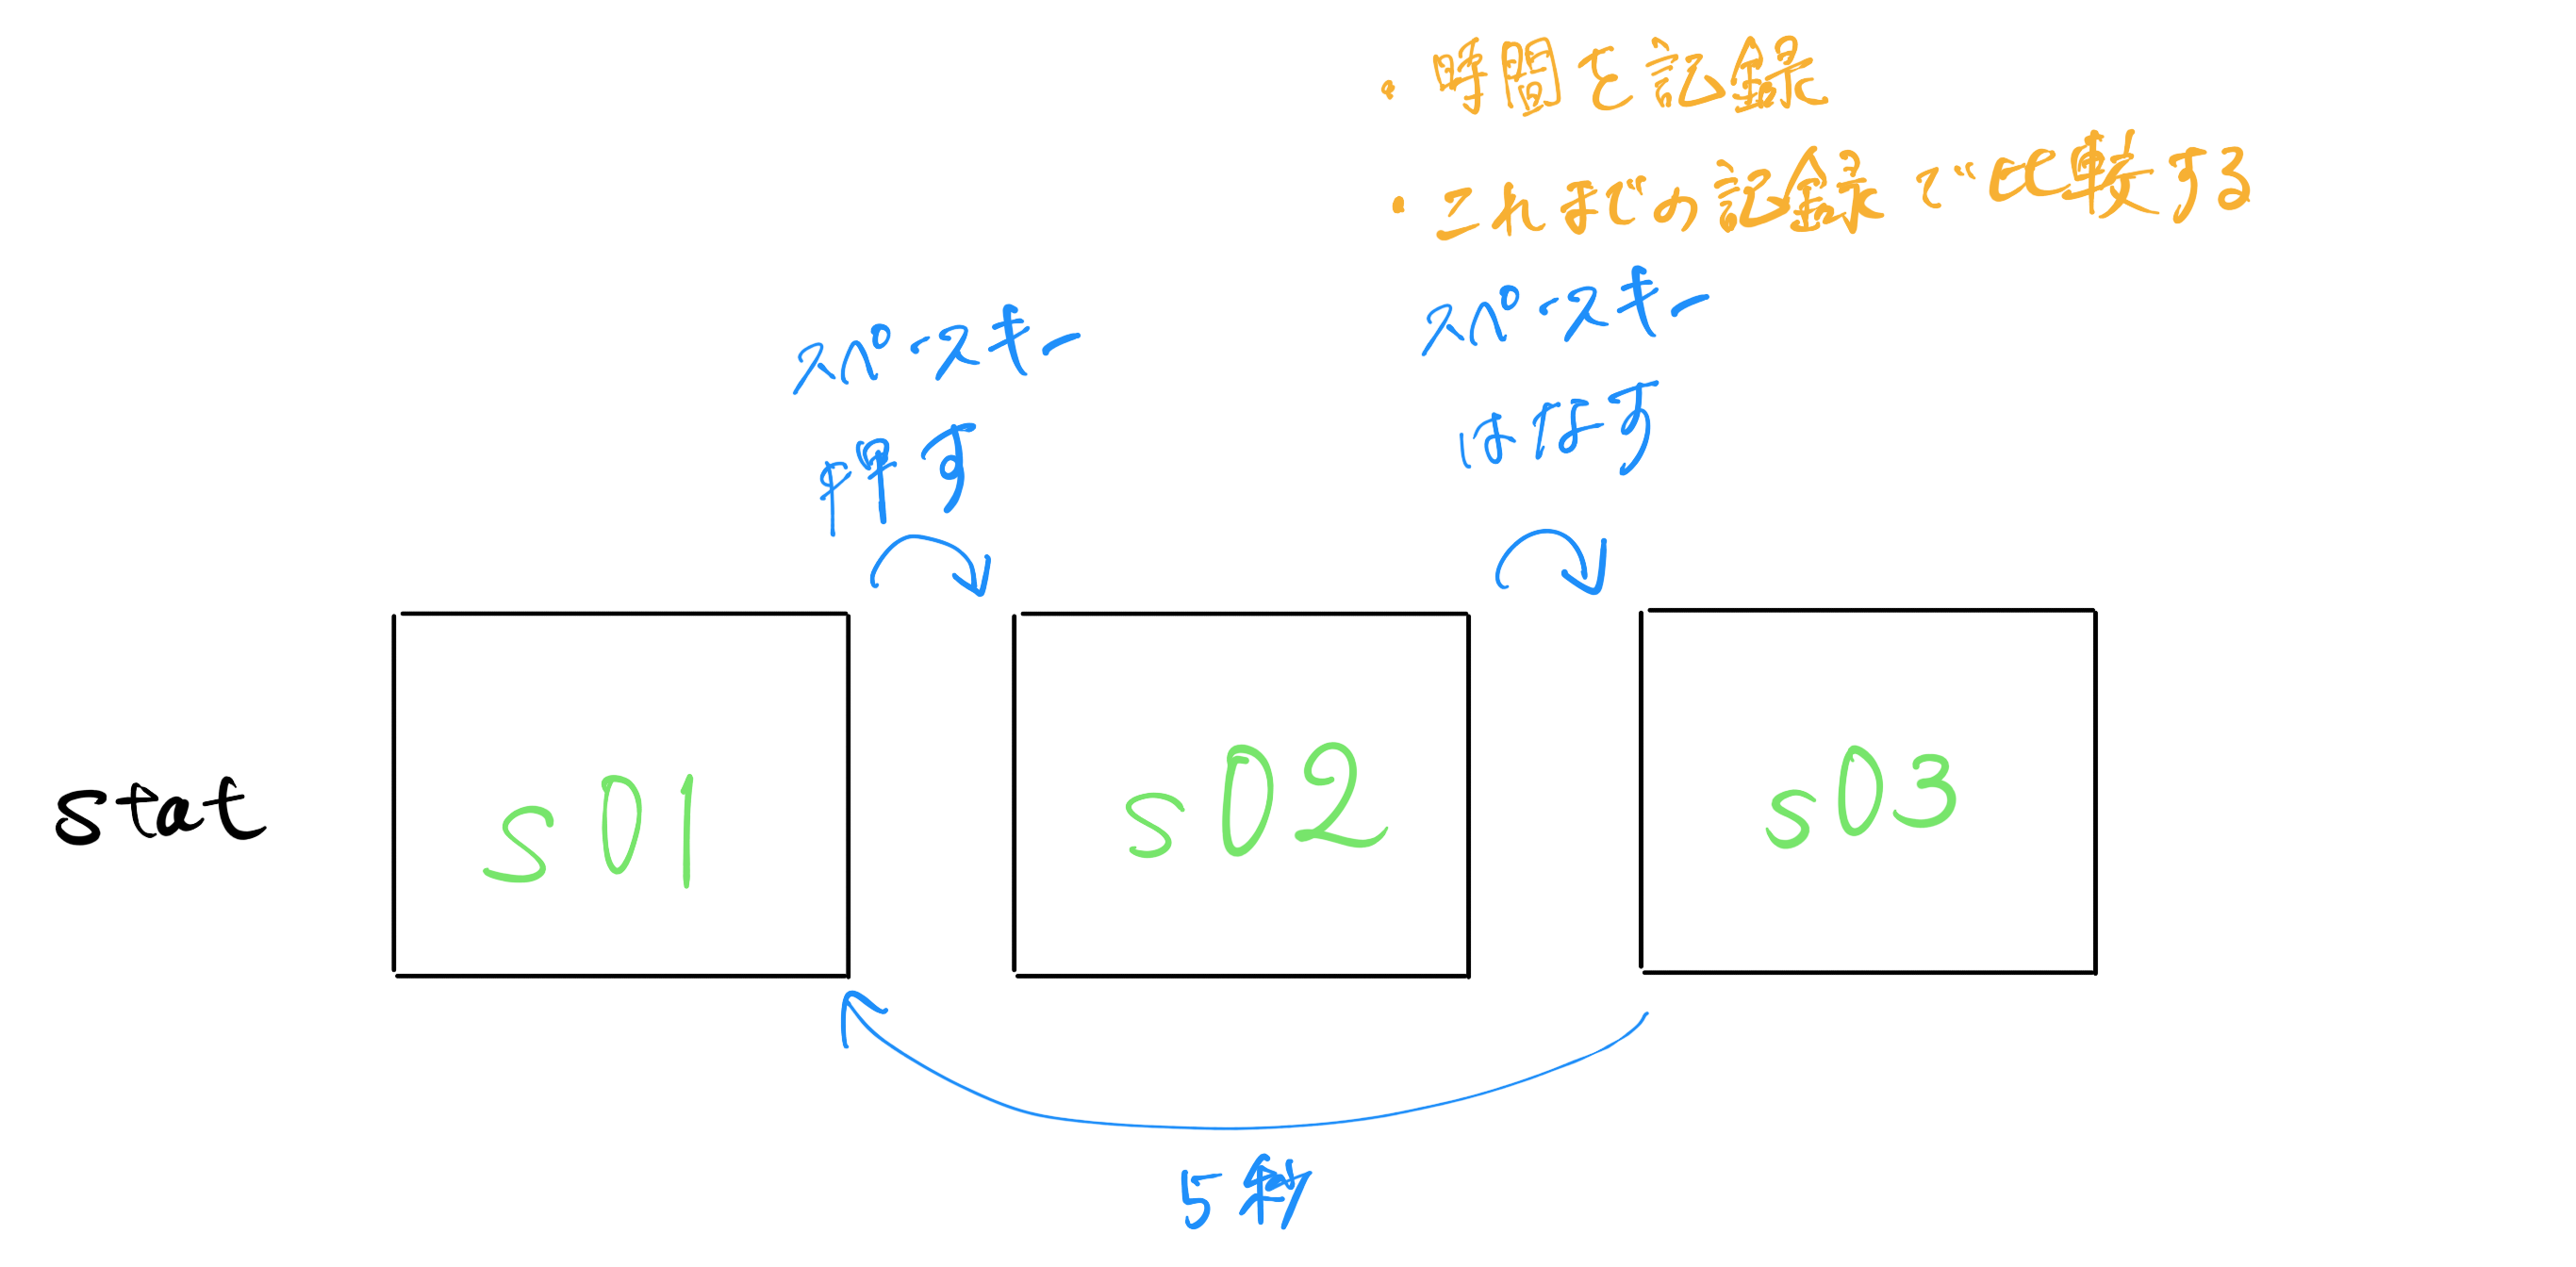
\includegraphics[width=110mm]{images/ws04-1.png}
                 \caption{WS04ステータス移行図解}
                \label{fig:15}
            \end{figure}
        \end{frame}

        \begin{frame}
            \frametitle{記録する,比べる WS04RecordCompare/}
            \begin{figure}[htb]
                 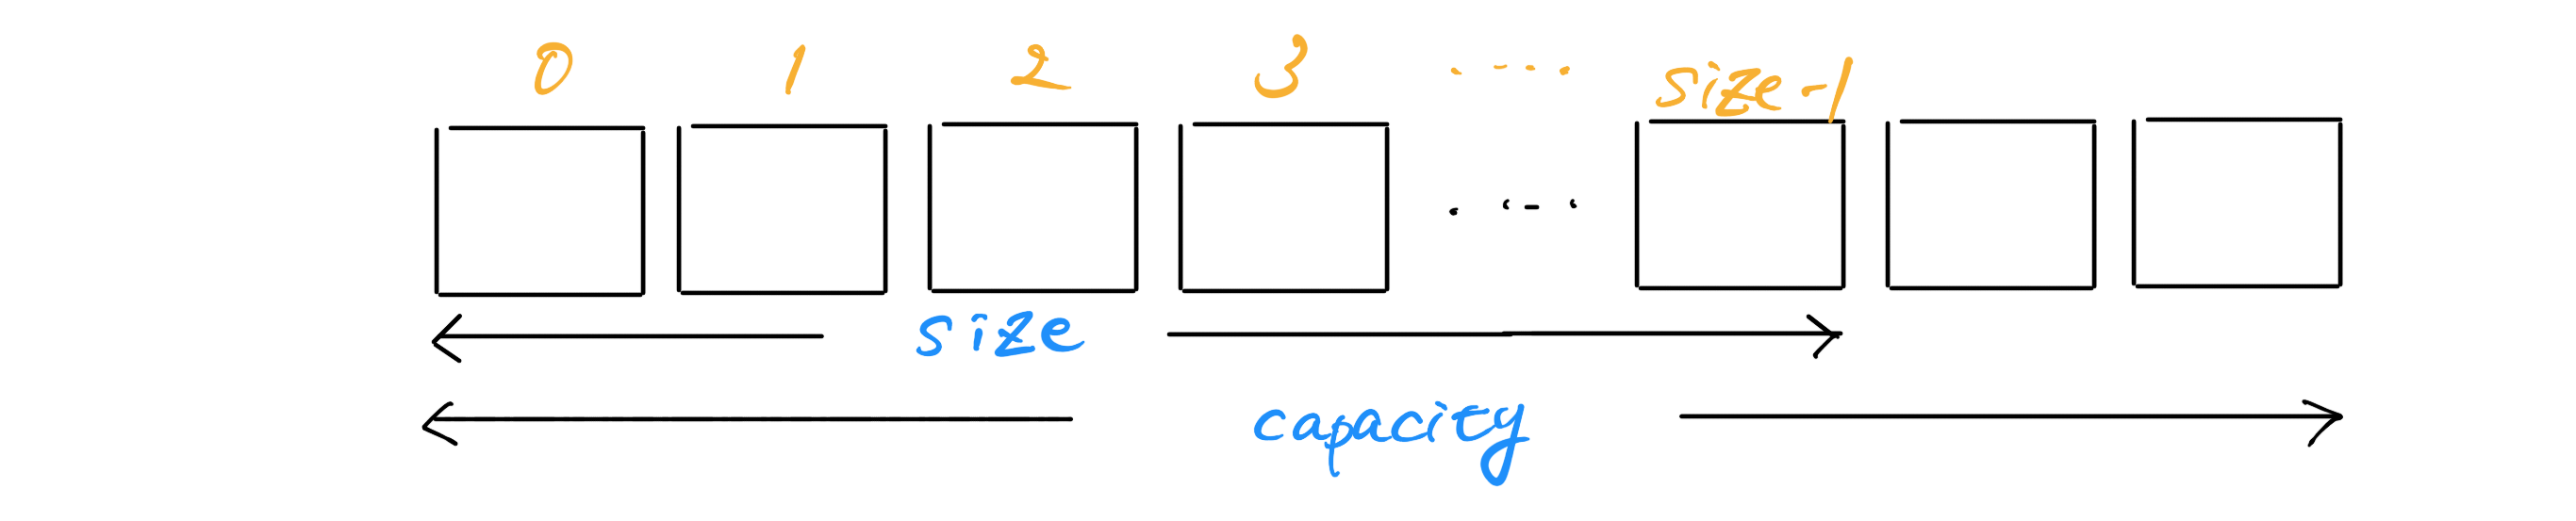
\includegraphics[width=110mm]{images/ws04-2.png}
                 \caption{動的配列}
                \label{fig:16}
            \end{figure}
        \end{frame}

        \begin{frame}
            \frametitle{リセット,削除 WS05Reset/}
            \begin{figure}[htb]
                 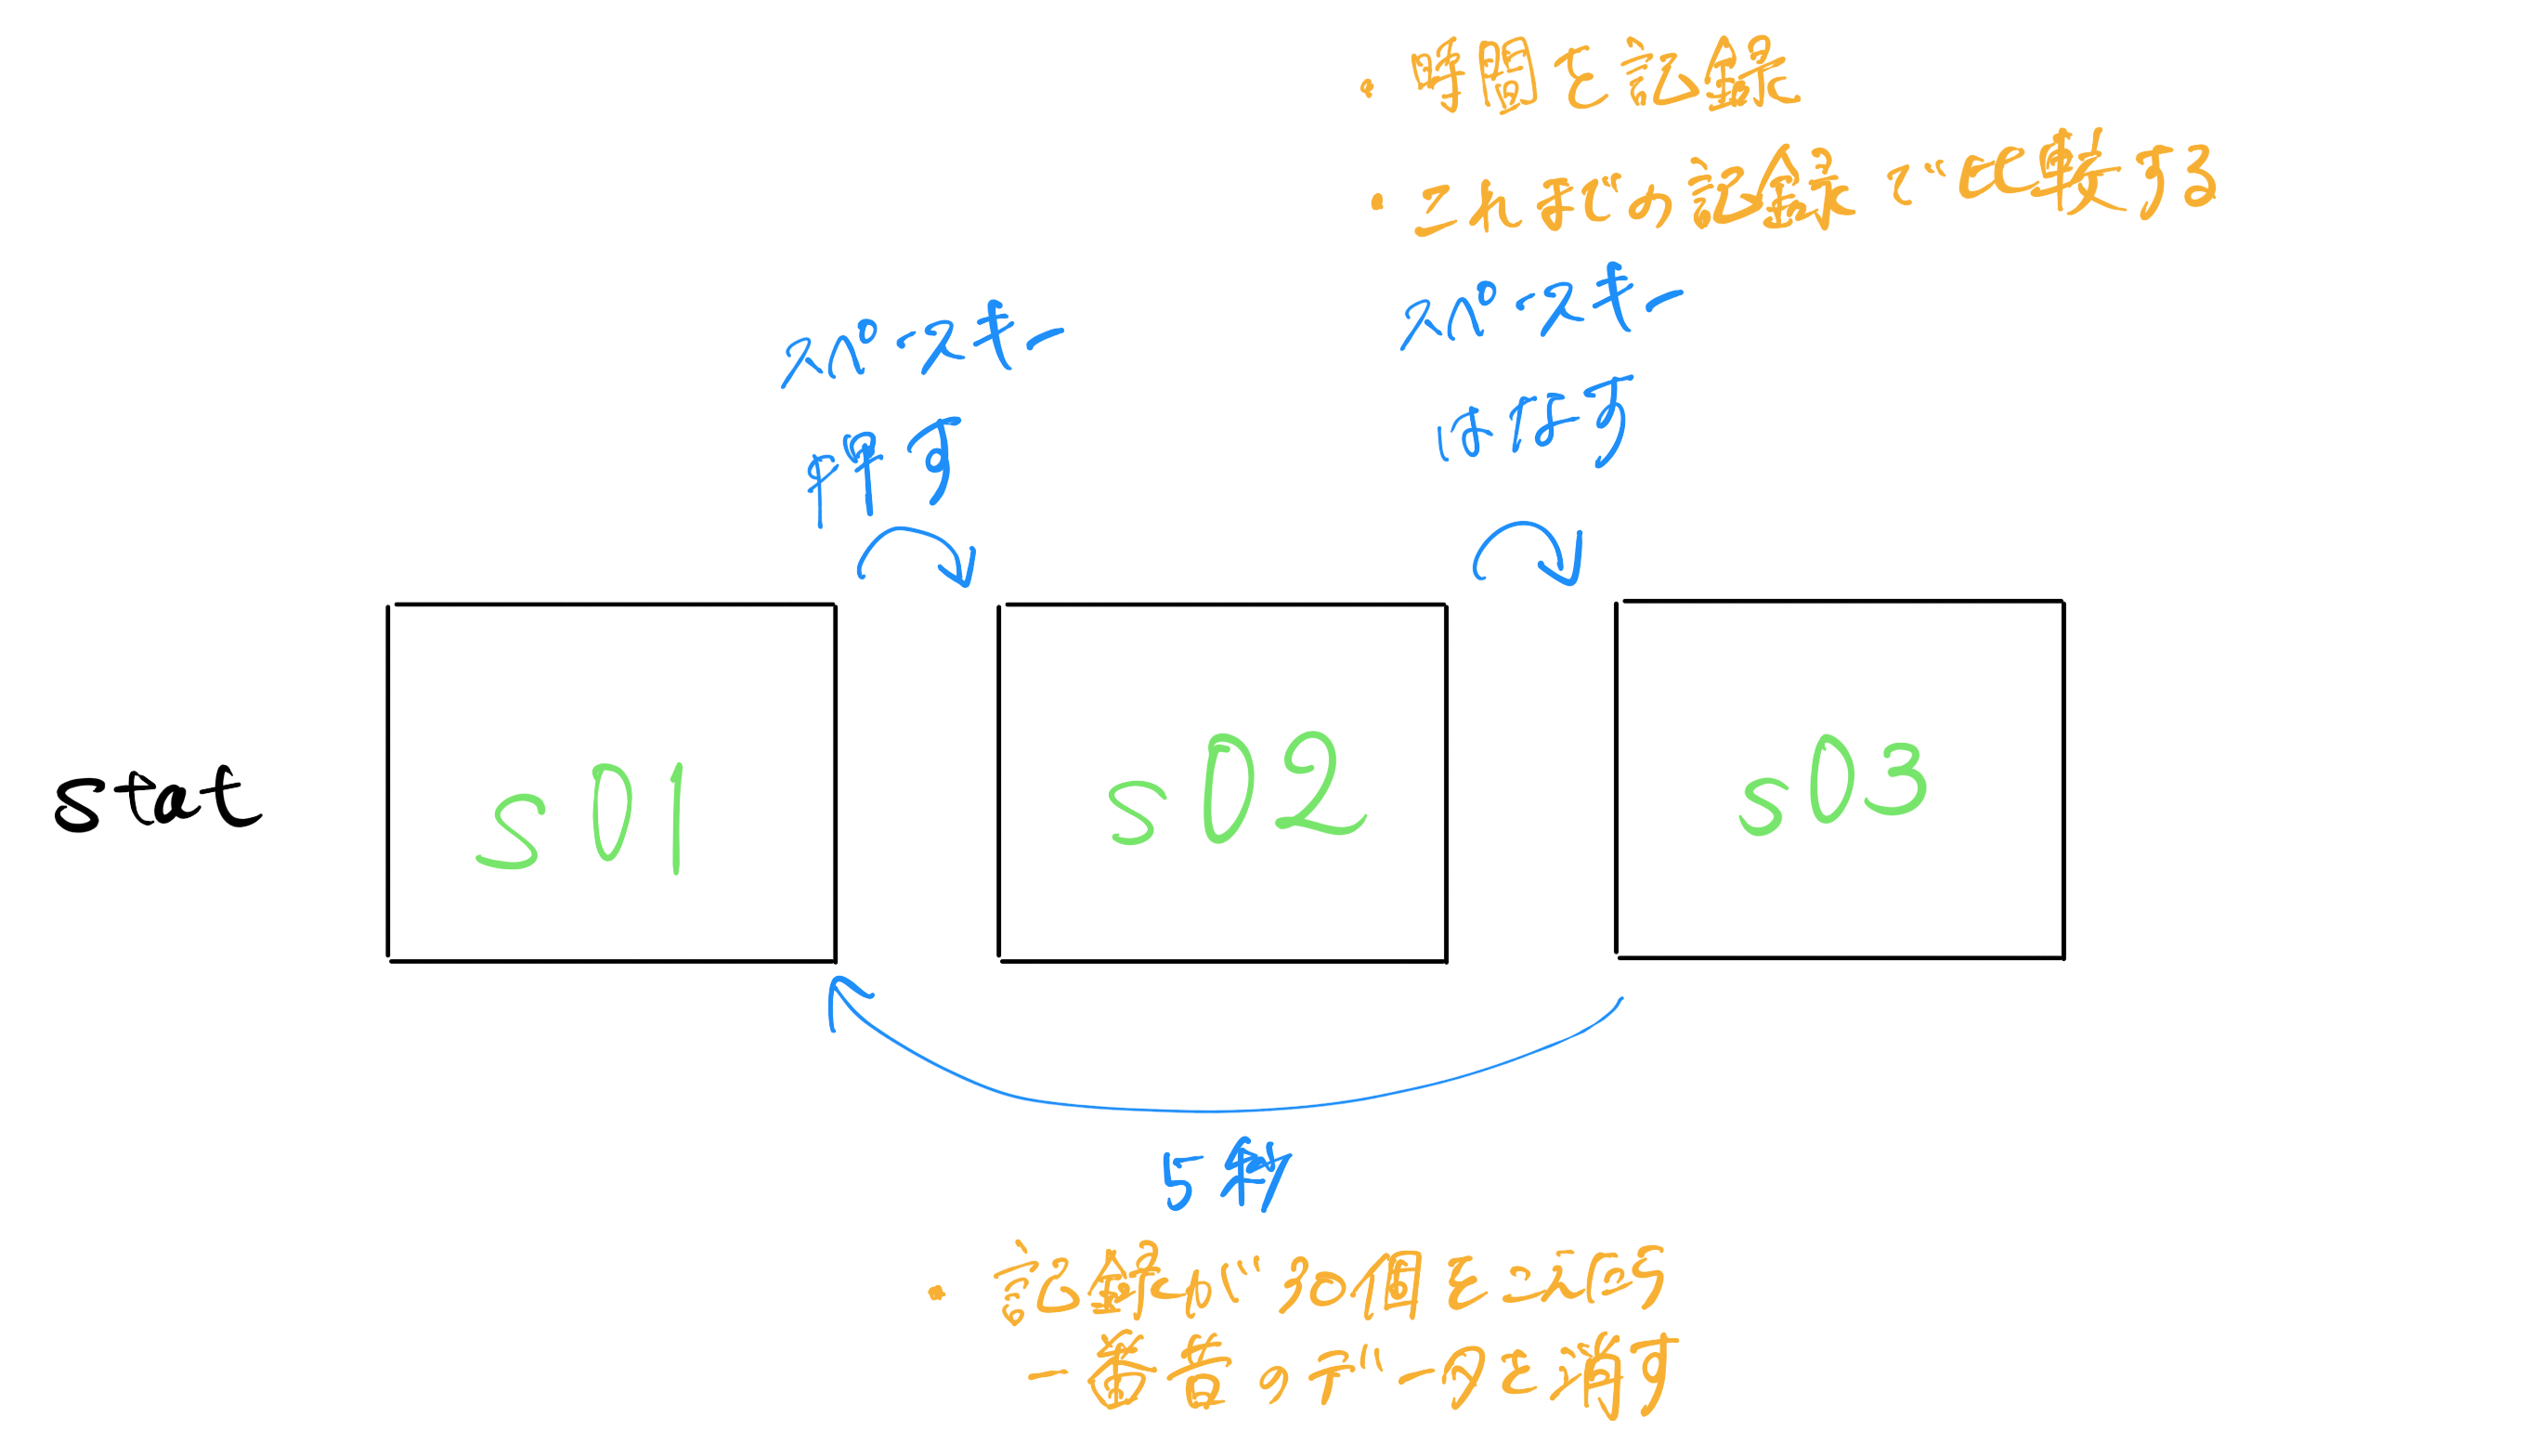
\includegraphics[width=110mm]{images/ws05-1.png}
                 \caption{WS05ステータス移行図解}
                \label{fig:17}
            \end{figure}
        \end{frame}

% 1日目4限:oFレクチャー
    \section{作品をフローチャートで書いてみる}
        \begin{frame}
            \centering{作りたい作品をフローチャートに起こしてみましょう}
        \end{frame}

        \begin{frame}
            \centering{共有タイム}
        \end{frame}
\end{document}

